% TU Delft beamer template
% Author: Erwin Walraven (initial version was created by Maarten Abbink)
% Delft Universiy of Technology

\documentclass{beamer}
\usepackage[english]{babel}
\usepackage{calc}
\usepackage[absolute,overlay]{textpos}
\usepackage{graphicx}
\usepackage{subfig}
\usepackage{amsmath}
\usepackage{amsfonts}
\usepackage{amsthm}
\usepackage{braket}
\usepackage{epstopdf}

\usepackage{comment}
\usepackage{MnSymbol,wasysym}

\setbeamertemplate{navigation symbols}{} % remove navigation symbols
\mode<presentation>{\usetheme{tud}}

% BIB SETTINGS
\usepackage[backend=bibtex,firstinits=true,maxnames=30,maxcitenames=20,url=false,style=authoryear]{biblatex}
\bibliography{bibfile}
\setlength\bibitemsep{0.3cm} % space between entries in the reference list
\renewcommand{\bibfont}{\normalfont\scriptsize}
\setbeamerfont{footnote}{size=\tiny}
\renewcommand{\cite}[1]{\footnote<.->[frame]{\fullcite{#1}}}


\title[]{Quantum Trajectories and Decoherence}
\institute[]{Delft University of Technology, The Netherlands}
\author{Bas Dirkse \and Jaap Wesdorp}
%\date{}

\begin{document}
{
\setbeamertemplate{footline}{\usebeamertemplate*{minimal footline}}
\frame{\titlepage}
}

{\setbeamertemplate{footline}{\usebeamertemplate*{minimal footline}}

}

\begin{frame}{Outline}
\begin{itemize}
	\item Open quantum systems
	\item Model of environment interaction
	\item Monte Carlo Algorithm
	\item Von Neumann Entropy
	\item Microscopic Trajectories
	\item Discussion
\end{itemize}
\end{frame}

\section{Introduction to noise}
\begin{frame}{Open quantum systems}
	\begin{itemize}
		\item Open versus closed quantum system
		\item Evolution of state by non-unitary operator and discontinuous `quantum jumps'
		\item 	\emph{``A Description of open quantum systems in terms of a statistical average over single realizations"}
	\end{itemize}
\end{frame}
	
\begin{frame}{The Lindblad Master equation}
	$$
	\dot{\rho}(t) = -i [H,\rho] + \sum_j  \gamma_j ( 2 F_j \rho F_j^\dagger - F_j^\dagger F_j \rho - \rho F_j^\dagger F_j  )
	$$
Which leads to
$$
H_{eff} = H_0 - i \sum_j \gamma_j F_j^\dagger F_j, 
$$
$$
S = \sum S_j, \quad S_j := \gamma F_j \rho F_j^\dagger
$$

$F_j$ are the quantum jump operators.
\end{frame}


\begin{frame}{Monte Carlo evolution of open quantum system}
	General idea
	\begin{itemize}
		\item Start with a pure state $\ket{\psi}$ 
		\item An imaginary observer sees if a quantum jump $F_j$ occurred during time $\Delta t$ 
		\begin{itemize}
			\item If not, state evolves continuously (but non-unitarilly) with non-hermitian Hamiltonian $H_{eff}$;
			\item Or the state discontinuously jumps to state $F_j \ket{\psi}$
		\end{itemize}
		\item Evolve until time final time $T$
		\item Repeat process $N$ times from same initial state $\ket{\psi}$ and compute ensemble average $\rho$
	\end{itemize}
\end{frame}


\begin{frame}{Monte Carlo evolution of open quantum system}
		Algorithm 
		\begin{enumerate}
			\item initiate state $\ket{\psi}$
			\item Compute probability $p_j = \gamma_j \Delta t \braket{\psi | F_j^\dagger F_j | \psi} $ of jump
			\item Choose integer $i \in \{0,1,2,...\}$ with probability $(1 - \sum_j p_j), p_1, p_2,...$
			\item If $i = 0$:  $\ket{\psi} \leftarrow \exp(-iH_{eff}\Delta t)\ket{\psi}$
			\item Else: $\ket{\psi} \leftarrow F_i \ket{\psi}$
			\item Renormalize: $\psi \leftarrow \frac{\ket{\psi}}{\sqrt{\braket{\psi|\psi}}}$ and go to 2 
			\item repeat 1-6 for $N$ times to obtain an ensemble average
		\end{enumerate}
\end{frame}

\begin{frame}{(De)coherence : Von neumann entropy}
	Measure of "known" information
	\begin{equation}
	S = -Tr(\rho \text{ln}\rho)
	\end{equation}
	\begin{figure}
		\centering
		\includegraphics[width=0.7\textwidth]{figs/von_neumann_5.jpeg}
	\end{figure}
\end{frame}

\begin{frame}{What did we model?}
	\begin{itemize}
		\item A two-level system (qubit) in $\mathcal{H}_2$ split by an energy difference $\hbar \omega$
		\item The Hamiltonian of the closed system is then $H = \frac{\hbar \omega}{2} \sigma_z$
		\item We initialize our system in the pure state $\ket{\psi} = \ket{+} = \frac{1}{\sqrt{2}} (\ket{0} + \ket{1})$
		\item We modeled different possible quantum jumps $F_j$ and examined their individual trajectories as well as their ensemble average.
	\end{itemize}
\end{frame}


\section{Microscopic Trajectories}
\begin{frame}{Microscopic Trajectories: Excited state relaxation}
	Two level system which decays to ground state.
	Jump operator taken as (lowering)ladder operator applied to initial state.
	\begin{figure}[h]
		\centering
		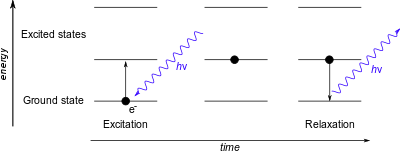
\includegraphics[width=0.6\textwidth]{figs/relaxation.png}
		\label{fig:digraph}
	\end{figure}
\end{frame}


\begin{frame}{Microscopic Trajectories: Excited state relaxation}
	
	\begin{figure}[!htb]
		\centering
		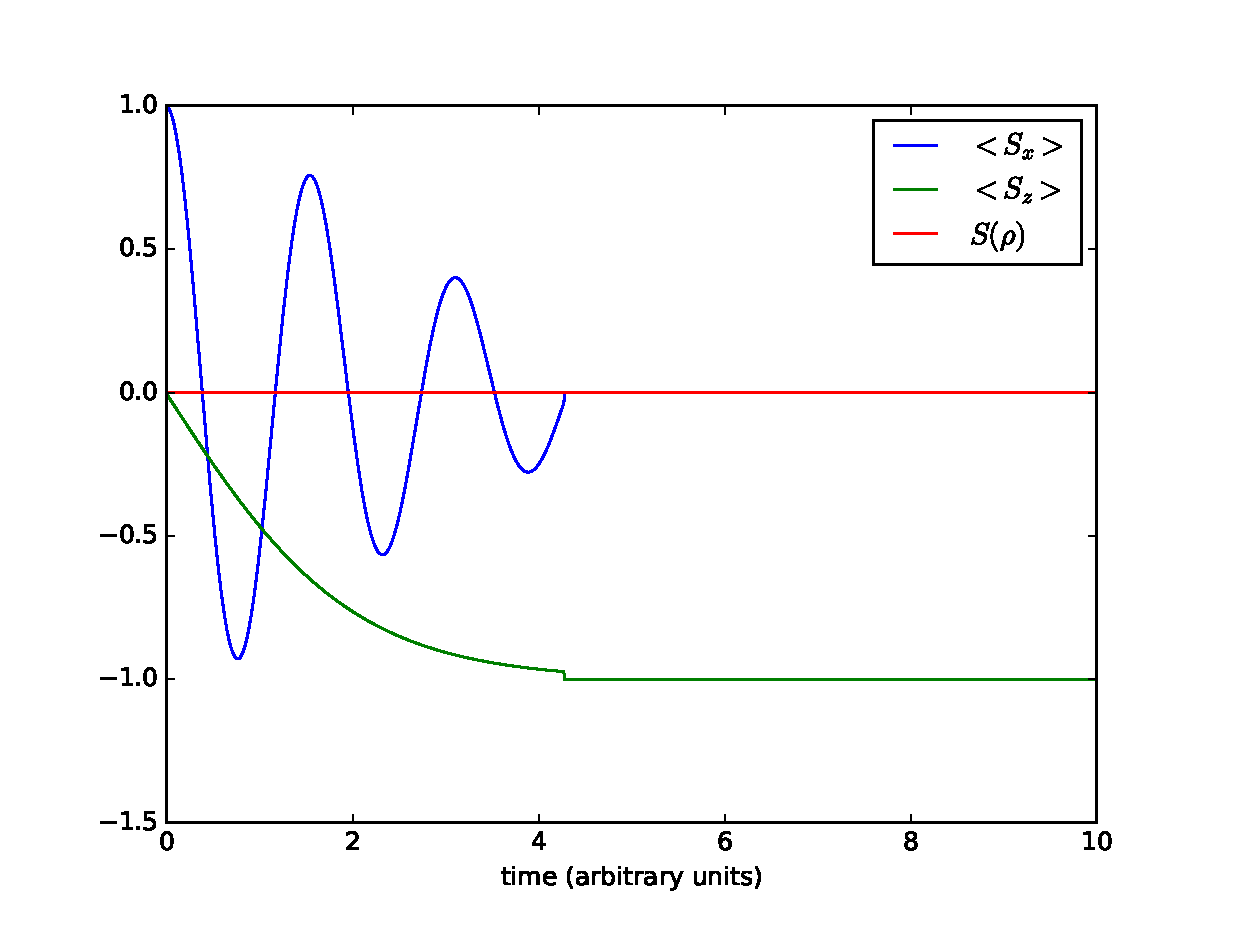
\includegraphics[width=0.7\textwidth]{figs/relaxation_1.eps}
	\end{figure}
		\begin{equation*}
		F_1 = \sigma_- =
		\begin{pmatrix}
		0 & 1 \\
		0 & 0 
		\end{pmatrix}
		\end{equation*}
\end{frame}
\begin{frame}{Entropy : Relaxation average}
	\begin{figure}[h]
		\centering
		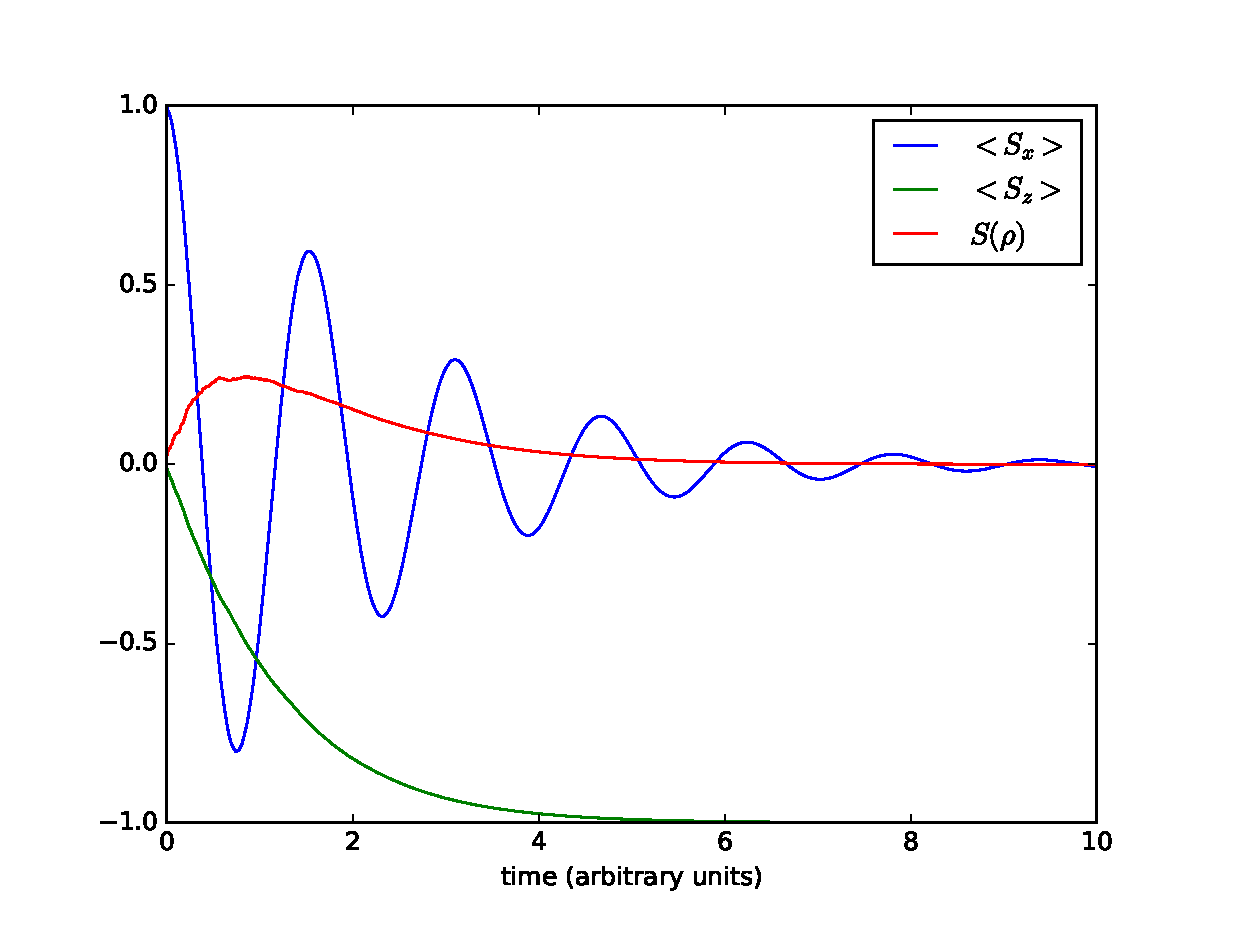
\includegraphics[width=0.7\textwidth]{figs/relaxation_1000.eps}
	\end{figure}
\end{frame}
\begin{frame}{Entropy :  Unequal relaxation / excitation times}
	\begin{figure}[h]
		\centering
		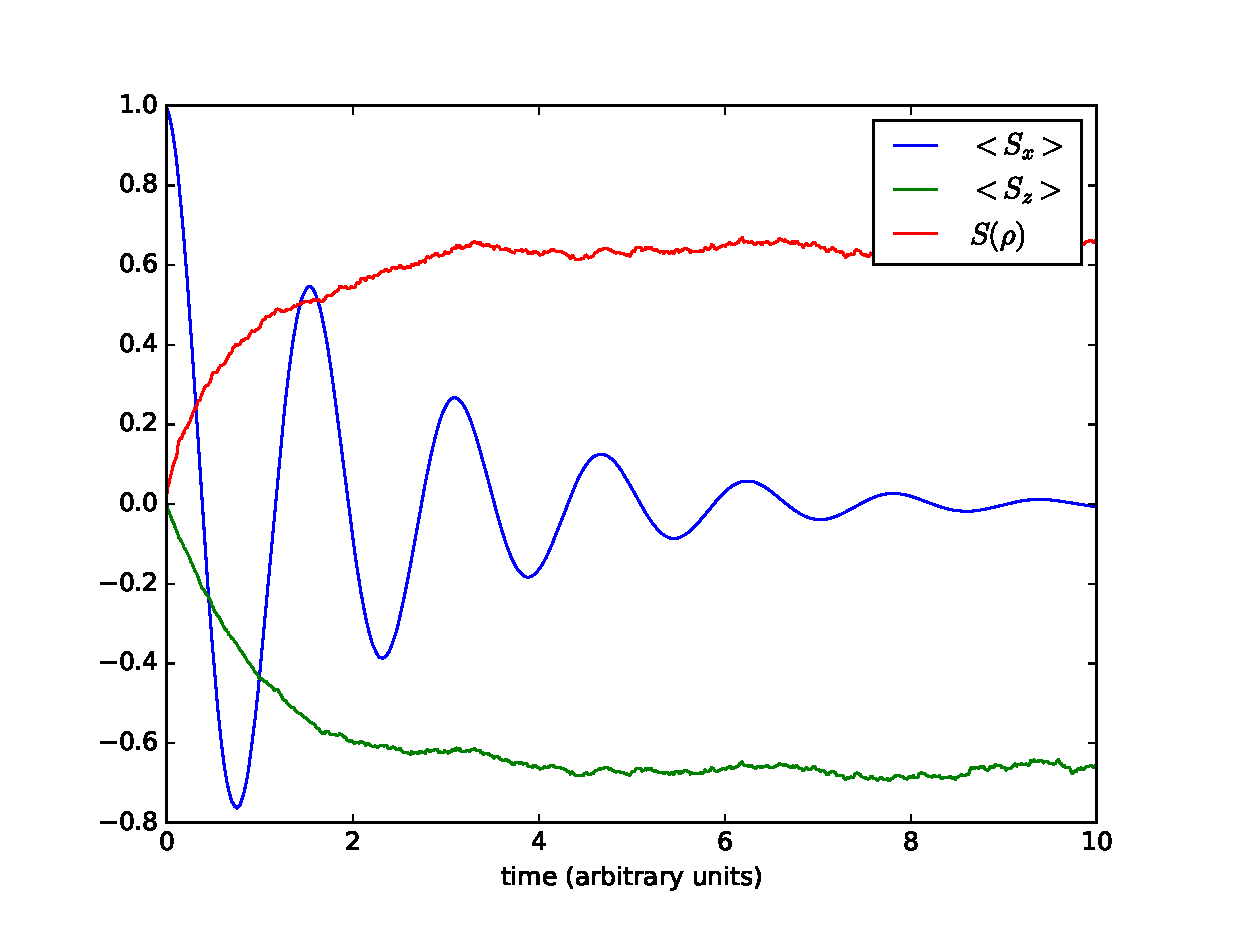
\includegraphics[width=0.7\textwidth]{figs/unequal_bitflip_1000.eps}
	\end{figure}
\end{frame}
\begin{frame}{Entropy: Equal relaxation / excitation times }
	Boson bath in thermal equilibrium
	\begin{figure}[h]
		\centering
		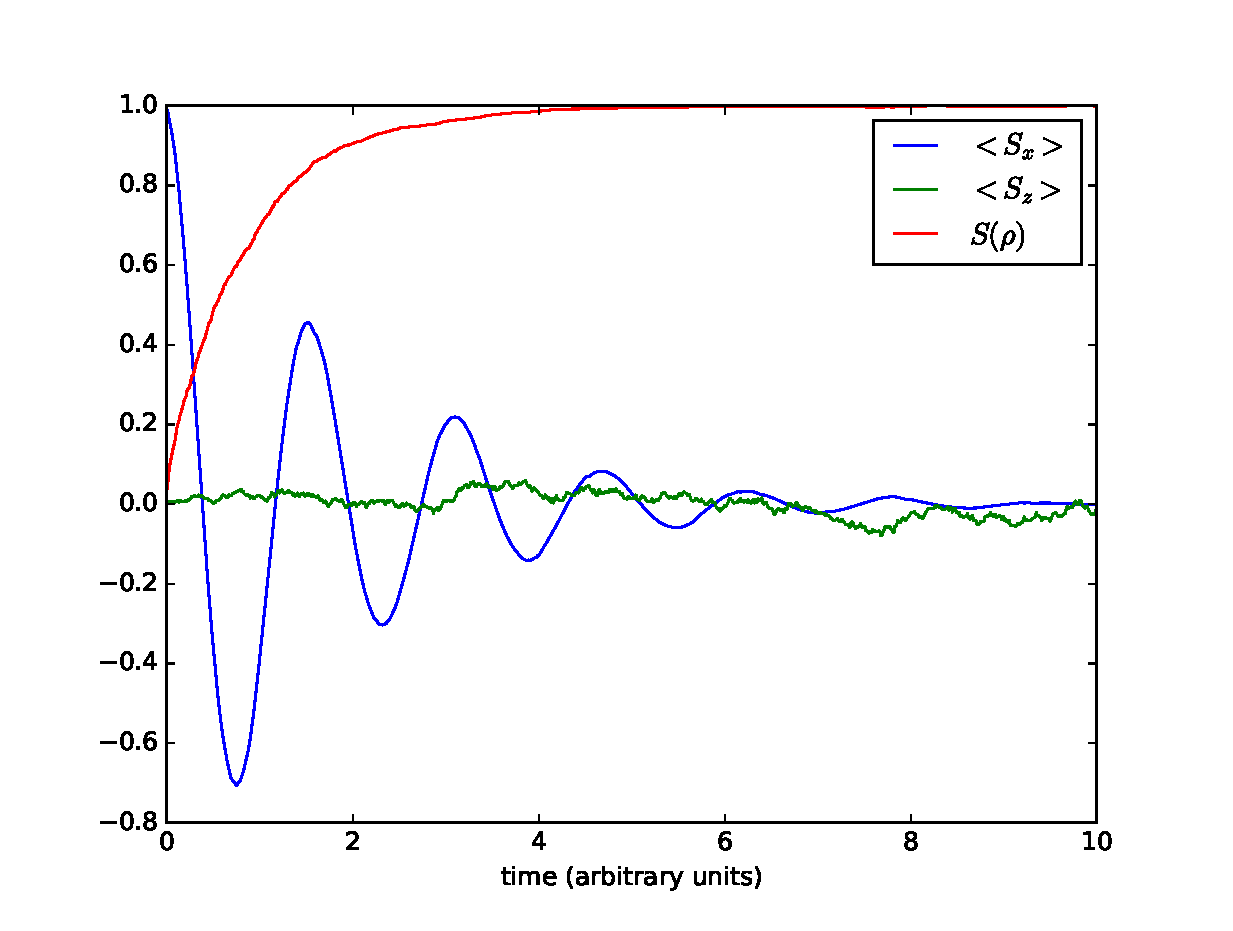
\includegraphics[width=0.7\textwidth]{figs/equal_bitflip_1000.eps}
	\end{figure}
\end{frame}

\begin{frame}{Microscopic Trajectories: Random phase kick}
	\begin{figure}[h]
		\centering
		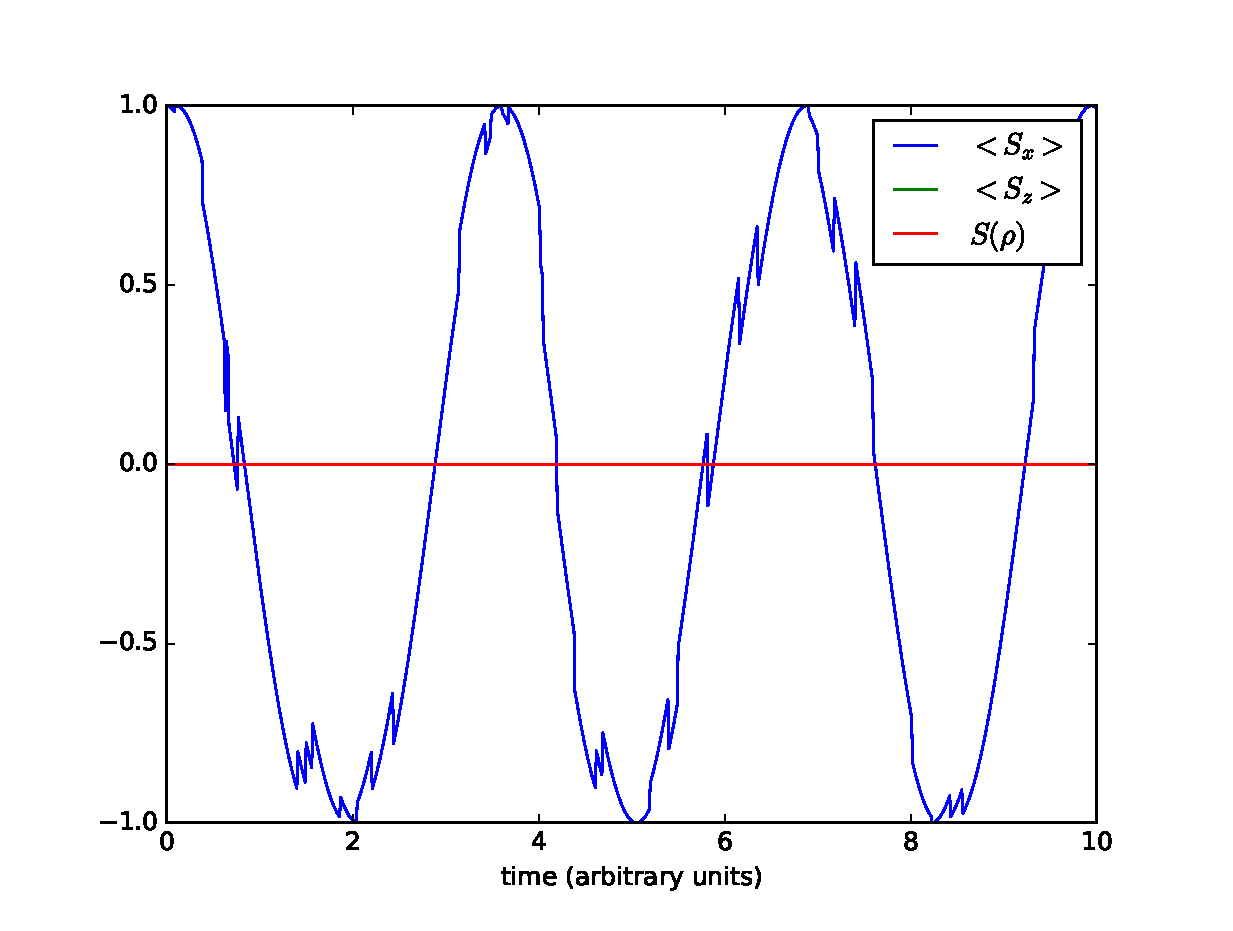
\includegraphics[width=0.7\textwidth]{figs/phase_jump_1.eps}
	\end{figure}
	\begin{equation*}
	F_1 =
	\begin{pmatrix}
	1 & 0 \\
	0 & e^{i\theta} 
	\end{pmatrix},\hspace{20pt}
	F_2 = 
	\begin{pmatrix}
	1 & 0 \\
	0 & e^{-i\theta} 
	\end{pmatrix}
	\end{equation*}
\end{frame}

\begin{frame}{Entropy :  Random phase kick average}
	\begin{figure}[h]
		\centering
		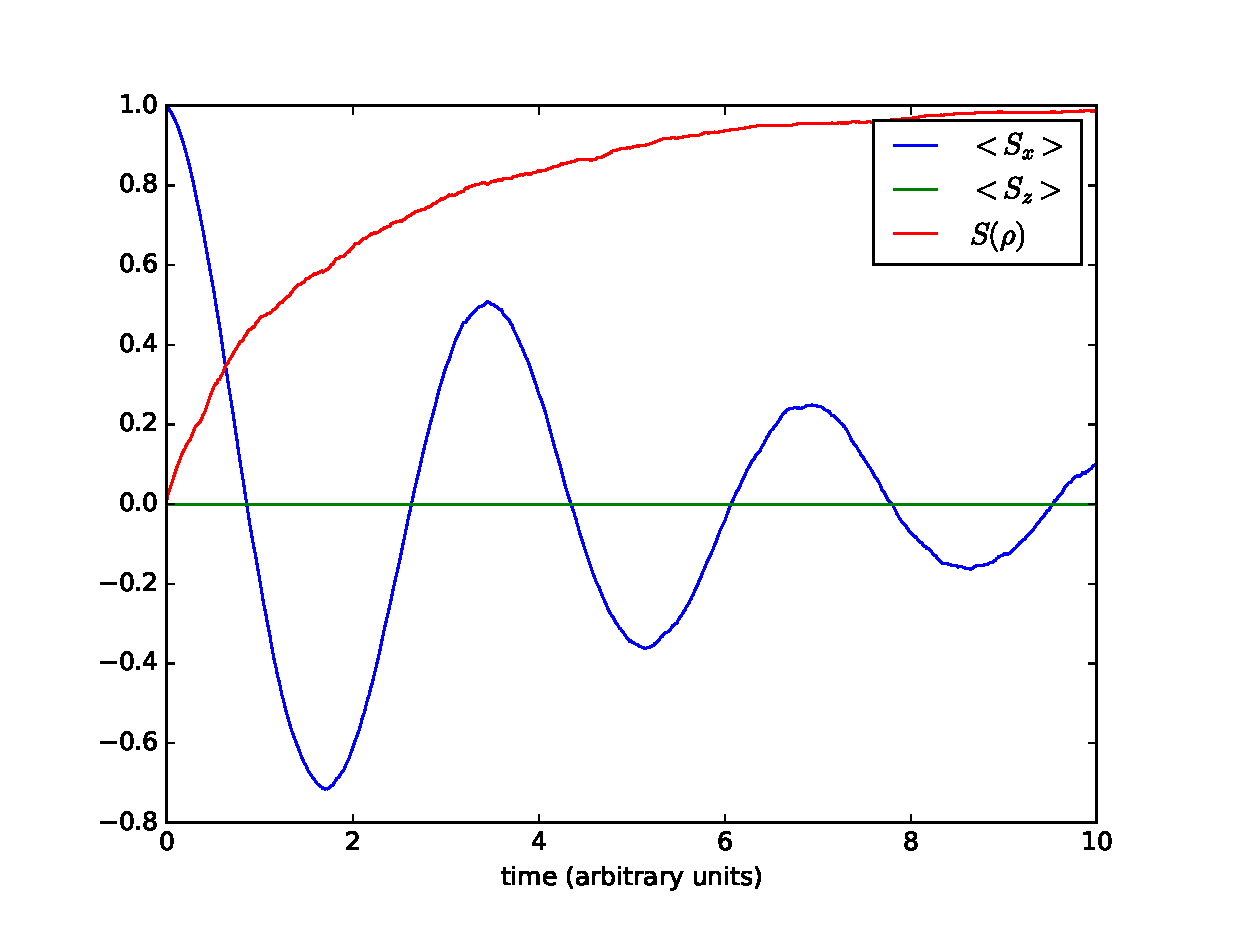
\includegraphics[width=0.7\textwidth]{figs/phase_jump_1000.eps}
	\end{figure}
\end{frame}

\begin{frame}{Microscopic Trajectories: Phase flip}
	\begin{figure}[h]
		\centering
		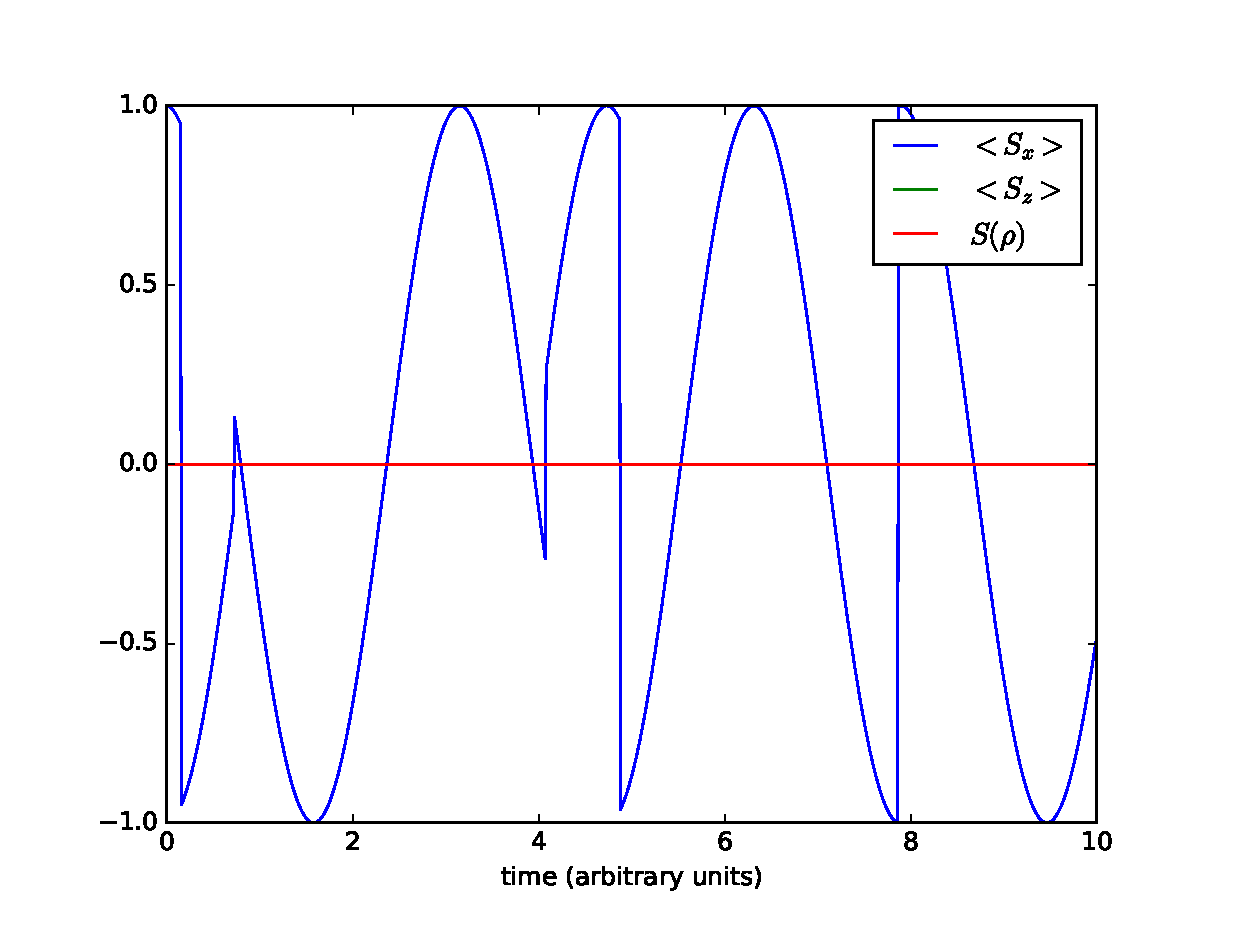
\includegraphics[width=0.7\textwidth]{figs/phase_flip_1.eps}
	\end{figure}
	\begin{equation*}
	F_1 = S_z =
	\begin{pmatrix}
	1 & 0 \\
	0 & -1 
	\end{pmatrix}
	\end{equation*}
\end{frame}

\begin{frame}{Entropy :  Phase flip average}
	\begin{figure}[h]
		\centering
		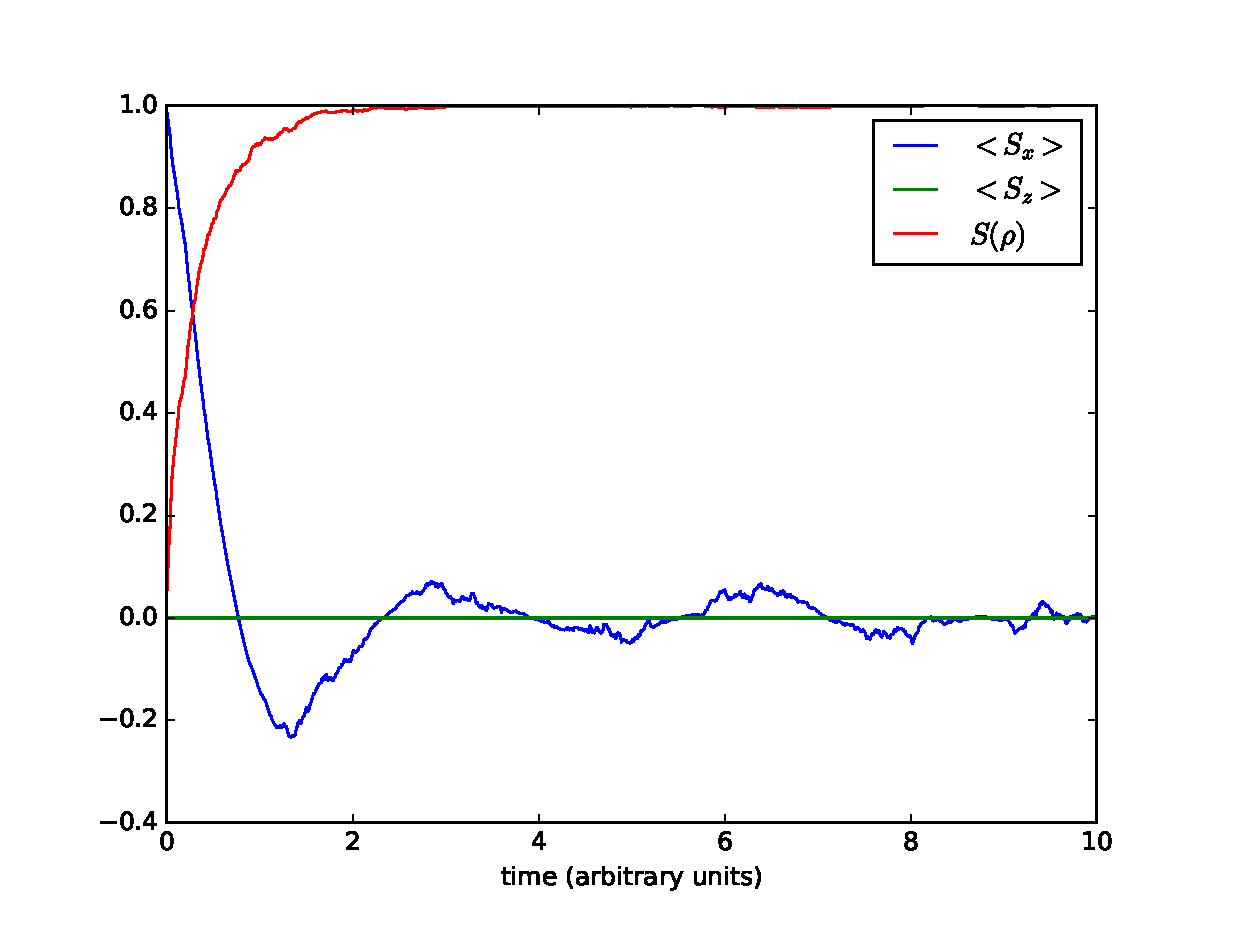
\includegraphics[width=0.7\textwidth]{figs/phase_flip_1000.eps}
	\end{figure}
\end{frame}

\begin{frame}{Freedom of interpretation}
	\begin{equation*}
	2\rho = 
	\begin{pmatrix}
	1 & 0 \\
	0 & 1
	\end{pmatrix}=
	\ket{0}\bra{0} \hspace{2pt} + \hspace{2pt}\ket{1}\bra{1}=\ket{+}\bra{+} \hspace{2pt}+ \hspace{2pt}\ket{-}\bra{-}
	\end{equation*}
	\begin{enumerate}
		\item Density matrix can be unraveled in many ways
		\item Different microscopic density matrix evolution for same exponential decoherence of pure state.
		\item \emph{There exists no measurement that can distinguish between the different phase damping processes}
	\end{enumerate}
\end{frame}

\end{document}
